\newcommand{\ee}{\mathrm{e}}
\newcommand{\ii}{\mathrm{i}}
\heading{数学物理方法（上）-第15次作业}

\begin{question}
证明Laplace变换的性质，其中 \(f(t) \to F(p)\)，对于前三个定理，写出Fourier变换的类似结论

1. 延迟定理 \(f(t-t_0) \eta(t-t_0) \to \ee^{-p t_0} F(p)\)；
2. 平移定理 \(\ee^{p_0 t} f(t) \eta(t) \to F(p-p_0)\)；
3. 相似定理 \(f(a t) \eta(t) \to \frac1a F(p/a),\quad a>0\)；
4. \(\displaystyle\int_t^\infty \frac{f(\tau)}{\tau}\dd{}\tau\, \eta(t) \to \frac1p \int_0^p F(q)\dd{q}\)。

\begin{solution}
1. \(\displaystyle\mathcal{L}\{f(t-t_0) \eta(t-t_0)\} = \int_{t_0}^\infty f(t-t_0)\ee^{-p t}\dd{t} = \ee^{-p t_0}\int_0^\infty f(t) \ee^{-p t}\dd{t} = \ee^{-p t_0} F(p)\)。其对应的Fourier变换类似结论是 \(\displaystyle\mathcal{F}\{f(x-x_0)\} = \int_{-\infty}^\infty \ee^{-\ii k x} f(x-x_0)\dd{x} = \ee^{-\ii k x_0} F(k)\)。
2. \(\displaystyle\mathcal{L}\{\ee^{p_0 t} f(t) \eta(t)\} = \int_0^\infty f(t) \ee^{-(p-p_0) t}\dd{t} = F(p-p_0)\)。其对应的Fourier变换类似结论是 \(\displaystyle\mathcal{F}\{\ee^{\ii k_0 x} f(x)\} = \int_{-\infty}^\infty \ee^{-\ii (k-k_0) x} f(x)\dd{x} = F(k-k_0)\)。
3. \(\displaystyle\mathcal{L}\{f(a t) \eta(t)\} = \int_0^\infty f(a t) \ee^{-p t}\dd{t} = \int_0^\infty f(u) \ee^{-p/a u}\,\frac{du}{a} = \frac1a F(p/a)\)。其对应的Fourier变换类似结论是 \(\displaystyle\mathcal{F}\{f(a x)\} = \int_{-\infty}^\infty \ee^{-\ii k x} f(a x)\dd{x} = \int_{-\infty}^\infty \ee^{-\ii k/a u} f(u)\,\frac1a\dd{u} = \frac1a F(k/a),\quad a>0\)。
4. 对等号左边作拉普拉斯变换 \[ \mathcal{L}\Bigl\{\int_t^\infty \frac{f(\tau)}{\tau}\dd{}\tau\,\eta(t)\Bigr\} = \int_0^\infty \int_t^\infty \frac{f(\tau)}{\tau}\dd{}\tau\, \ee^{-p t}\dd{t} \]对积分顺序作变换有 \[ \mathcal{L}\Bigl\{\int_t^\infty \frac{f(\tau)}{\tau}\dd{}\tau\,\eta(t)\Bigr\} = \int_0^\infty \frac{f(\tau)}{\tau} \int_0^\tau \ee^{-p t}\dd{t}\dd{}\tau = \int_0^\infty \frac{f(\tau)}{\tau}\cdot\frac{1-\ee^{-p\tau}}{p}\dd{}\tau \]对于等号右边，有 \[ \frac1p \int_0^p F(q)\dd{q} = \frac1p \int_0^p \int_0^\infty f(t) \ee^{-q t}\dd{t}\dd{q} = \frac1p \int_0^\infty \frac{f(t)}{t} (1-\ee^{-p t})\dd{t} \]作变量替换 \(t\to\tau\)，可以发现两者相等，即 \(\displaystyle\int_t^\infty \frac{f(\tau)}{\tau}\dd{}\tau\,\eta(t) \to \frac1p \int_0^p F(q)\dd{q}\)。

\begin{center}
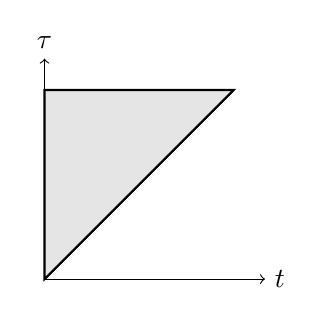
\begin{tikzpicture}[scale=0.8]
  \draw[->] (0,0) -- (3.5,0) node[right] {$t$};
  \draw[->] (0,0) -- (0,3.5) node[above] {$\tau$};
  \draw[thick] (0,0) -- (3,3);
  \draw[thick,fill=black!10] (0,0) -- (3,3) -- (0,3) -- cycle;
\end{tikzpicture}
\end{center}
\end{solution}
\end{question}

\begin{question}
求下列函数的Laplace换式：
1. \(t^\alpha,\ \operatorname{Re}\alpha >-1\);
2. \(t-a\lfloor t/a\rfloor,\ a>0\);
3. \(\dfrac{1-\cos\omega t}{t^2},\ \omega>0\);
4. \(\displaystyle\int_t^\infty \frac{\sin\tau}{\tau}\dd{}\tau\).
\begin{solution}

1. 即计算积分 \(\displaystyle\int_0^\infty \ee^{-p t} t^{\alpha}\dd{t}\)。作换元 \(\tau = p t\)，有 \[ \mathcal{L}\{t^\alpha\}=\int_0^\infty \ee^{-\tau} (\tau/p)^{\alpha}\,\frac{d\tau}{p} = \frac{\Gamma(\alpha+1)}{p^{\alpha+1}} \]

2. 即计算积分 \(\displaystyle\int_0^\infty (t-a\lfloor t/a\rfloor) \ee^{-p t}\dd{t}\)。分段积分，有 \[ \mathcal{L}\{t-a\lfloor t/a\rfloor\} = \sum_{n=0}^\infty \int_{n a}^{(n+1) a} (t-n a) \ee^{-p t}\dd{t} = \sum_{n=0}^\infty \int_0^a t \ee^{-p (t+n a)}\dd{t} \] \[ = \frac{1}{1-\ee^{-p a}} \int_0^a t \ee^{-p t}\dd{t} = \frac{1}{1-\ee^{-p a}}\frac{1-\ee^{-p a}(p a+1)}{p^2} \]

3. 利用像函数积分的反演公式 \(\displaystyle\frac{f(t)}{t} \to \int_p^\infty F(q)\dd{q}\)，有 \[ \mathcal{L}\{1-\cos\omega t\}=\frac1p-\frac12\frac1{p+\ii\omega}-\frac12\frac1{p-\ii\omega} \] \[ \mathcal{L}\Bigl\{\frac{1-\cos\omega t}{t}\Bigr\} = \int_p^\infty \Bigl(\frac1q-\frac12\frac1{q+\ii\omega}-\frac12\frac1{q-\ii\omega}\Bigr)\dd{q} = \frac12\ln\frac{p^2+\omega^2}{p^2} \] \[ \mathcal{L}\Bigl\{\frac{1-\cos\omega t}{t^2}\Bigr\} = \int_p^\infty \frac12\ln\frac{q^2+\omega^2}{q^2}\dd{q} = \frac12 p\ln\frac{p^2}{p^2+\omega^2}+\omega\arctan\frac{\omega}{p} \]

4. 根据 Problem 1中所证明的，\[ \int_t^\infty \frac{\sin\tau}{\tau}\dd{}\tau \to \frac1p \int_0^p \frac{1}{p^2+1}\dd{p} = \frac1p \arctan p \]
\end{solution}
\end{question}

\begin{question}
求下列函数的Fourier换式：（下列各式中 \(a>0\)）

1. \(\Pi_a(x)=\begin{cases}0 & |x|>a/2,\\ 1 & |x|<a/2\end{cases}\);
2. \(\ee^{-x^2/a^2}\);
3. \(\operatorname{Ш}_a(x)=\displaystyle\sum_{n=-\infty}^\infty \delta(x-n a)\).
\begin{solution}
1. \(\displaystyle\mathcal{F}\{\Pi_a(x)\} = \frac1{\sqrt{2\pi}}\int_{-a/2}^{a/2} \ee^{-\ii k x}\dd{x} = \sqrt{\frac2\pi}\frac{\sin(k a/2)}{k}\)。

2. \(\displaystyle\mathcal{F}\{\ee^{-x^2/a^2}\} = \frac1{\sqrt{2\pi}}\int_{-\infty}^\infty \ee^{-x^2/a^2-\ii k x}\dd{x} = \frac{\ee^{-a^2 k^2/4}}{\sqrt{2\pi}}\int_{-\infty}^\infty \ee^{-(x/a-\ii a k/2)^2}\dd{x} = \frac{a}{\sqrt2} \ee^{-a^2 k^2/4}\)

3. \(\displaystyle\mathcal{F}\{\operatorname{Ш}_a(x)\} = \frac1{\sqrt{2\pi}}\sum_{n=-\infty}^\infty \ee^{-\ii k n a}\)。当 \(k\neq \dfrac{2q\pi}{a}\) 时，求和显然为 \(0\)。对于一般的情况，我们考察极限过程 \[ \lim_{N\to+\infty}\frac1{\sqrt{2\pi}}\sum_{-N}^N \ee^{-\ii k a\cdot n}= \lim_{N\to+\infty}\frac1{\sqrt{2\pi}}\frac{\sin\bigl(k a(1/2+N)\bigr)}{\sin(k a/2)} = \sum_{q=-\infty}^\infty \sqrt{\frac{\pi}{2}}\,\delta\Bigl(\frac{k a}{2}-q\pi\Bigr) \]
\end{solution}
\end{question}

\begin{question}
求下列 Laplace 换式的原函数：
1. \(\dfrac{\ee^{-p\tau}}{p^2},\ (\tau>0)\);

2. \(\dfrac1p\dfrac{\ee^{-\alpha p}}{1-\ee^{-\alpha p}},\ (\alpha>0)\);
3. \(\dfrac{\ee^{-p\tau}}{p^4+4\omega^4},\ (\tau>0,\ \omega>0)\);
4. \(\dfrac1p\dfrac{\cosh(l-x)\sqrt p}{\cosh l\sqrt p},\ (0<x<l)\).
\begin{solution}

1. 有 \(\displaystyle\mathcal{L}\{t\} = \int_0^\infty t \ee^{-p t}\dd{t} = \frac1{p^2}\)，因此有 \(\displaystyle\mathcal{L}\{(t-\tau)\eta(t-\tau)\} = \frac{\ee^{-p\tau}}{p^2}\)，故 \(\displaystyle\frac{\ee^{-p\tau}}{p^2} \gets (t-\tau)\eta(t-\tau)\)。

2. 有 \(\displaystyle\frac1p\frac{\ee^{-\alpha p}}{1-\ee^{-\alpha p}} = \frac1p\bigl[\ee^{-\alpha p}+\ee^{-2\alpha p}+\dots\bigr] \gets \sum_{n=1}^\infty \eta(t-n\alpha) = \lfloor t/\alpha\rfloor\)。

3. 有 \[ \frac1{p^4+4\omega^4} = \frac1{8\omega^3}\Bigl[\frac1{-1+\ii}\frac1{p-\omega(1+\ii)}+\frac1{-1-\ii}\frac1{p-\omega(1-\ii)}+\frac1{1+\ii}\frac1{p-\omega(-1+\ii)}+\frac1{1-\ii}\frac1{p-\omega(-1-\ii)}\Bigr] \]因此其拉普拉斯变换为 \[ \frac1{p^4+4\omega^4} \gets \frac1{8\omega^3}\Bigl[\frac{\ee^{\omega(1+\ii)t}}{-1+\ii}+\frac{\ee^{\omega(1-\ii)t}}{-1-\ii}+\frac{\ee^{\omega(-1+\ii)t}}{1+\ii}+\frac{\ee^{\omega(-1-\ii)t}}{1-\ii}\Bigr] \] \[ = -\frac1{16\omega^3}\bigl((1+\ii)\ee^{\omega(1+\ii)t}+(1-\ii)\ee^{\omega(1-\ii)t}+(-1+\ii)\ee^{\omega(-1+\ii)t}+(-1-\ii)\ee^{\omega(-1-\ii)t}\bigr) \] \[ =\frac1{4\omega^3}\bigl[\sin(\omega t)\cosh(\omega t)-\cos(\omega t)\sinh(\omega t)\bigr] \]因此有，\[ \frac{\ee^{-p\tau}}{p^4+4\omega^4} \gets \frac1{4\omega^3}\bigl[\sin(\omega(t-\tau))\cosh(\omega(t-\tau))-\cos(\omega(t-\tau))\sinh(\omega(t-\tau))\bigr]\eta(t-\tau) \]

4. 使用一般的反演变换公式，有 \(\displaystyle f(t)=\frac1{2\pi\ii}\int_{s-\ii\infty}^{s+\ii\infty} F(p) \ee^{p t}\dd{p}\)，考察围道

\begin{center}
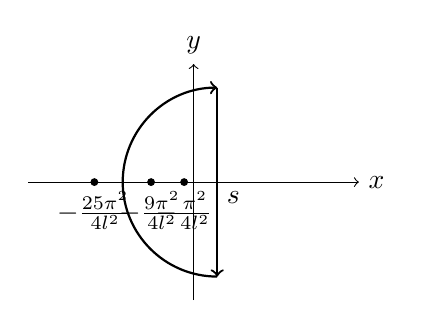
\begin{tikzpicture}[scale=0.6]
  \draw[->] (-3.5,0) -- (3.5,0) node[right] {$x$};
  \draw[->] (0,-2.5) -- (0,2.5) node[above] {$y$};
  % Bromwich contour: vertical line Re(p)=s plus large circular arc to the left
  \draw[thick,->] (0.5,2) -- (0.5,-2);
  \draw[thick,->] (0.5,-2) arc (-90:-270:2);
  % Mark branch points on negative real axis
  \filldraw (-0.2,0) circle (2pt);
  \node at (-0.2,0) [below] {$-\frac{\pi^2}{4l^2}$};
  \filldraw (-0.9,0) circle (2pt);
  \node at (-0.9,0) [below] {$-\frac{9\pi^2}{4l^2}$};
  \filldraw (-2.1,0) circle (2pt);
  \node at (-2.1,0) [below] {$-\frac{25\pi^2}{4l^2}$};
  \node at (0.5,0) [below right] {$s$};
\end{tikzpicture}
\end{center}

\[ \oint_C \frac1{2\pi\ii}\frac1p\frac{\cosh(l-x)\sqrt p}{\cosh l\sqrt p} \ee^{p t}\dd{p} = \int_{C_R} \frac1{2\pi\ii}F(p)\ee^{p t}\dd{p} + \int_{s-\ii\infty}^{s+\ii\infty} \frac1{2\pi\ii}F(p)\ee^{p t}\dd{p} \]注意到，有 \(\displaystyle\lim_{p\to\infty}\frac1{2\pi\ii}\frac1p\frac{\cosh(l-x)\sqrt p}{\cosh l\sqrt p}=0\)，根据推广的Jordan引理，有 \(\displaystyle\lim_{R\to+\infty}\int_{C_R}\frac1{2\pi\ii}F(p)\ee^{p t}\dd{p}=0\)。而 \(F(p)\) 在 \(p=-\Bigl(\dfrac{\pi}{2l}\Bigr)^2(2n+1)^2,\ n\in\mathbb{N}\)，有 \[ \operatorname{res}\Bigl\{\frac1{\cosh l\sqrt p},\,-\Bigl(\frac{\pi(2n+1)}{2l}\Bigr)^2\Bigr\} = \frac{(-1)^n(2n+1)\pi}{l^2} \]因此有，\[ \operatorname{res}\Bigl\{\frac1{2\pi\ii}F(p)\ee^{p t},\,-\Bigl(\frac{\pi(2n+1)}{2l}\Bigr)^2\Bigr\} = \frac{(-1)^n}{2\pi\ii}\cos\Bigl(\frac{l-x}{l}(n+\tfrac12)\pi\Bigr)\frac4{\pi(2n+1)}\exp\Bigl(-\Bigl(\frac{\pi(2n+1)}{2l}\Bigr)^2 t\Bigr) \] \[ \operatorname{res}\Bigl\{\frac1{2\pi\ii}F(p)\ee^{p t},\,0\Bigr\} = \frac1{2\pi\ii} \]故可以得到 \[ \int_{s-\ii\infty}^{s+\ii\infty} \frac1{2\pi\ii}F(p)\ee^{p t} = 1 + \sum_{n=0}^\infty \frac{4(-1)^n}{\pi(2n+1)}\cos\Bigl(\bigl(1-\tfrac{x}{l}\bigr)(n+\tfrac12)\pi\Bigr)\exp\Bigl(-\Bigl(\frac{\pi(2n+1)}{2l}\Bigr)^2t\Bigr) \] \[ = 1- \frac4\pi\sum_{n=0}^\infty \frac1{2n+1}\exp\Bigl(-\Bigl(\frac{\pi(2n+1)}{2l}\Bigr)^2t\Bigr)\sin\Bigl(\frac{2n+1}{2l}\pi x\Bigr) \]
\end{solution}
\end{question}

\begin{question}
求下列Fourier换式的原函数：\(\cos(k a) F(k)\)，其中 \(F(k)=\mathcal{F}\{f(x)\}\)。
\begin{solution}
\[ \mathcal{F}\{f(x-a)\}=\ee^{-\ii k a}F(k),\quad \mathcal{F}\{f(x+a)\}=\ee^{\ii k a}F(k) \]因此有 \(\displaystyle\mathcal{F}^{-1}\{\cos(k a)F(k)\} = \frac12\bigl[f(x-a)+f(x+a)\bigr]\)。
\end{solution}
\end{question}

\begin{question}
利用Laplace变换计算下列积分：
1. \(\displaystyle\int_0^\infty \frac{\ee^{-a x}-\ee^{-b x}}{x}\cos c x\dd{x},\ a>0,\ b>0,\ c>0\);

2. \(\displaystyle\int_0^\infty \frac{1-\cos b x}{x^2}\dd{x},\ b>0\);

3. \(\displaystyle\int_0^\infty \frac{\sin x t}{x(x^2+1)}\dd{x}\).
\begin{solution}
1. \[ \ee^{-a x}\cos c x - \ee^{-b x}\cos c x \to \frac12\Bigl[\frac1{p+a+\ii c}+\frac1{p+a-\ii c}-\frac1{p+b+\ii c}-\frac1{p+b-\ii c}\Bigr] \]因此有 \[ \int_0^\infty \frac{\ee^{-a x}-\ee^{-b x}}{x}\cos c x\dd{x} = \int_0^\infty \frac12\Bigl[\frac1{p+a+\ii c}+\frac1{p+a-\ii c}-\frac1{p+b+\ii c}-\frac1{p+b-\ii c}\Bigr]dp \] \[ = \bigl.\frac12\ln\frac{(p+a)^2+c^2}{(p+b)^2+c^2}\bigr|_0^\infty = \frac12\ln\frac{b^2+c^2}{a^2+c^2} \]

2. \[ 1-\cos b x \to \frac1p-\frac12\frac1{p+\ii b}-\frac12\frac1{p-\ii b} \]因此有 \[ \frac{1-\cos b x}{x} \to \int_p^\infty \Bigl(\frac1p-\frac12\frac1{p+\ii b}-\frac12\frac1{p-\ii b}\Bigr)dp = \frac12\ln\frac{p^2+b^2}{p^2} \]故 \[ \int_0^\infty \frac{1-\cos b x}{x^2}\dd{x} = \int_0^\infty \frac12\ln\frac{p^2+b^2}{p^2}\dd{p} = \frac12\pi b \]

3. \[ \frac{\sin x t}{x(x^2+1)} \to \frac1{(x^2+1)(p^2+x^2)} \]因此有 \[ \int_0^\infty \frac{\sin x t}{x(x^2+1)}\dd{x} \to \int_0^\infty \frac1{(x^2+1)(p^2+x^2)}\dd{x} = \int_0^\infty \frac1{p^2-1}\Bigl[\frac1{x^2+1}-\frac1{x^2+p^2}\Bigr]dx = \frac{\pi}{2}\frac1{(p+1)p} \]而同时有 \(\displaystyle\frac1{p(p+1)} = \frac1p-\frac1{p+1} \gets 1-\ee^{-t}\)，因此上述结果为 \[ \int_0^\infty \frac{\sin x t}{x(x^2+1)}\dd{x} = \frac{\pi}{2}(1-\ee^{-t})\quad (t>0) \]而上述积分关于 \(t\) 为奇函数，因此有 \[ \int_0^\infty \frac{\sin x t}{x(x^2+1)}\dd{x} = \frac{\pi}{2}\operatorname{sgn}(t)(1-\ee^{-|t|}) \]
\end{solution}
\end{question}

\begin{question}
求解下列积分方程，其中 \(\alpha\) 为已知复数，\(f(t)\) 为已知函数，\(u(\xi)\) 是未知函数。\[ f(t)=\int_0^t \frac{u(\xi)}{(t-\xi)^\alpha}\dd{}\xi,\quad t>0,\ 0<\operatorname{Re}\alpha<1. \]
\begin{solution}
两边同时做拉普拉斯变换，左边等于 \(\mathcal{L}\{f(t)\}\)，右边利用卷积定理可以得到 \[ \mathcal{L}\Bigl\{\int_0^t \frac{u(\xi)}{(t-\xi)^\alpha}\dd{}\xi\Bigr\}=\mathcal{L}\{u(t)\}\mathcal{L}\{1/t^\alpha\}=\Gamma(1-\alpha)p^{\alpha-1}\mathcal{L}\{u(t)\} \]因此有 \[ \mathcal{L}\{u(t)\}=\frac{\mathcal{L}\{f(t)\}}{\Gamma(1-\alpha)p^{\alpha-1}} \ \Rightarrow\ u(t)=\mathcal{L}^{-1}\Bigl\{\frac{\mathcal{L}(f(t))}{\Gamma(1-\alpha)p^{\alpha-1}}\Bigr\} \]此时，再利用卷积定理，由 \(\displaystyle\frac1{p^\alpha} \gets \frac{t^{\alpha-1}}{\Gamma(\alpha)},\ pF(p) \gets \dv{f}{t}\) 可以得到 \[ u(t) = \int_0^t f'(\xi)\cdot\frac{(t-\xi)^{\alpha-1}}{\Gamma(1-\alpha)\Gamma(\alpha)}\dd{}\xi = \frac{\sin\pi\alpha}{\pi}\int_0^t f'(\xi)(t-\xi)^{\alpha-1}\dd{}\xi \]利用分部积分，有 \[ \int_0^t f'(\xi)(t-\xi)^{\alpha-1}\dd{}\xi =\bigl.f(\xi)(t-\xi)^{\alpha-1}\bigr|_0^t - \int_0^t f'(\xi)\dv{}{\xi}\bigl[(t-\xi)^{\alpha-1}\bigr]\dd{}\xi \] \[ = f(0)t^{\alpha-1} + \int_0^t \dv{}{t}\bigl[f'(\xi)(t-\xi)^{\alpha-1}\bigr]\dd{}\xi = \dv{}{t}\int_0^t f(\xi)(t-\xi)^{\alpha-1}\dd{}\xi \]因此最后有，\[ u(t)=\frac{\sin(\pi\alpha)}{\pi}\dv{}{t}\int_0^t f(\xi)(t-\xi)^{\alpha-1}\dd{}\xi \]
\end{solution}
\end{question}

\begin{question}
利用Laplace变换求解下列微分方程（组）或积分方程：
1. 如下图，合上开关 \(K\) 的时刻记为 \(t=0\)，已知 \(i(0)=0,\ q(0)=0\)，求 \(i(t)\)：

\begin{figure}
\centering
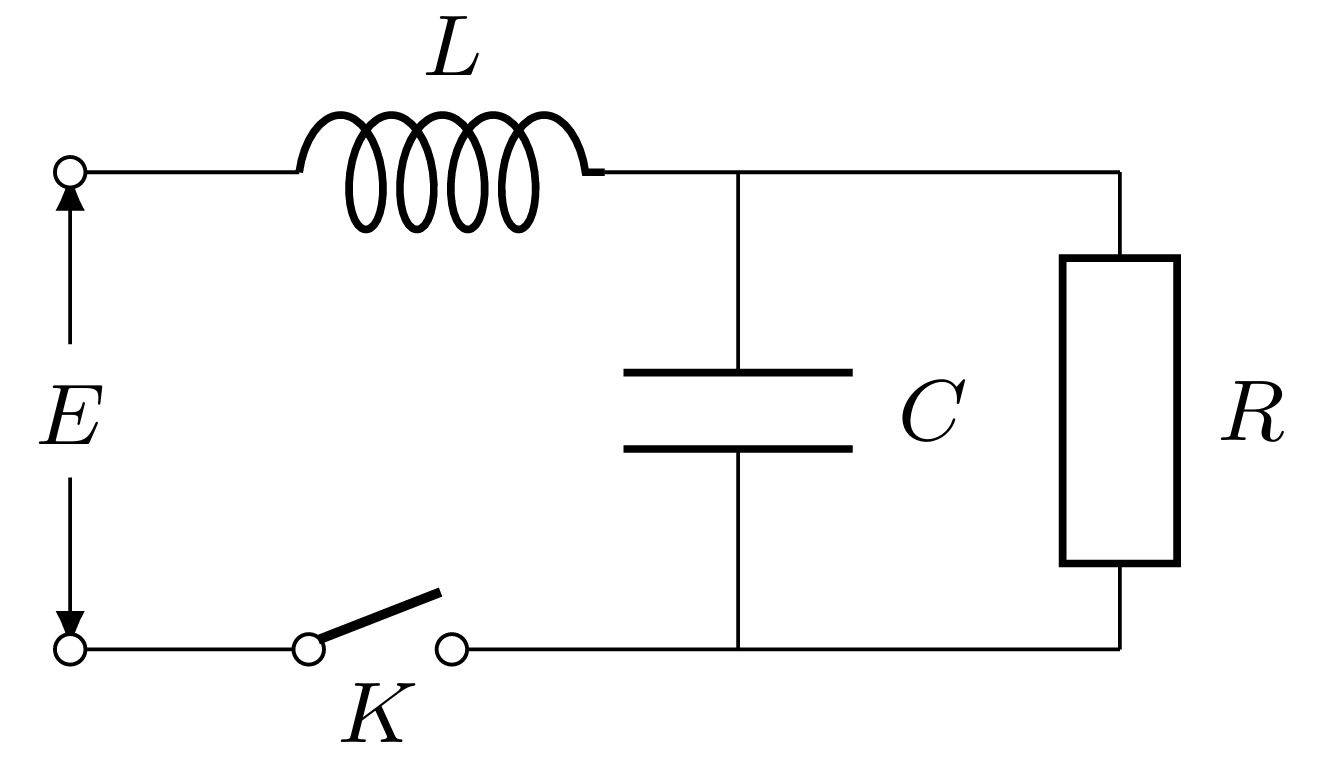
\includegraphics[width=5cm]{figures/image-2.png}
\caption{第8.(1)题图}
\end{figure}

2. \(f(t)+2\displaystyle\int_0^t f(\tau)\cos(t-\tau)\dd{}\tau=9\ee^{2t}\)
\begin{solution}
1. 设 \(C\) 上的电荷量为 \(q\)，\(R\) 上的电流为 \(i_0\)，则有干路电流 \(i=i_0+\dfrac{dq}{dt}\)，列出基尔霍夫方程组可以得到 \[ \begin{cases} E= q/C + L\dfrac{di}{dt},\\ q/C=(i-\dfrac{dq}{dt})R \end{cases} \]对等式两边作拉普拉斯变换，可以得到 \[ \begin{cases} E/p=Q(p)/C + L p I(p),\\ Q(p)/C=(I(p)-p Q(p))R \end{cases} \]解得 \[ Q(p)=\frac{E C R}{p(C L R p^2 +L p+R)},\quad I(p)=\frac{E (C R p+1)}{p(C L R p^2 +L p+R)} \]作反演变换可以得到 \[ q(t)=C E\Bigl[1+\frac{L-\sqrt{L(L-4 C R^2)}}{2\sqrt{L(L-4 C R^2)}}\ee^{-\frac{L+\sqrt{L(L-4 C R^2)}}{2 C L R}t}-\frac{L+\sqrt{L(L-4 C R^2)}}{2\sqrt{L(L-4 C R^2)}}\ee^{-\frac{L-\sqrt{L(L-4 C R^2)}}{2 C L R}t}\Bigr] \] \[ i(t)=\frac{E}{R}\Bigl[1+\frac{L-2 C R^2-\sqrt{L(L-4 C R^2)}}{2\sqrt{L(L-4 C R^2)}}\ee^{-\frac{L+\sqrt{L(L-4 C R^2)}}{2C L R}t}-\frac{L-2 C R^2+\sqrt{L(L-4 C R^2)}}{2\sqrt{L(L-4 C R^2)}}\ee^{-\frac{L-\sqrt{L(L-4 C R^2)}}{2C L R}t}\Bigr] \]

2. 两边作拉普拉斯变换，并且使用卷积定理，可以得到 \[ F(p) + 2F(p)\frac{p}{p^2+1} = \frac{9}{p-2} \]由此解得 \(F(p)=\dfrac{9(p^2+1)}{(p-2)(p+1)^2}\)，作反演变换可以得到 \(f(t)=(4-6t)\ee^{-t}+5\ee^{2t}\)。
\end{solution}
\end{question}

\begin{question}
利用 Laplace 变换，求解下列常微分方程边值问题：
\[ \dv[2]{y}{x}-k^2 y(x)=\delta(x-x'),\quad x>0,\ k>0,\ x'>0, \] \[ y'(0)=0,\ \bigl.y\bigr|_{x\to\infty}=0 \]
\begin{solution}
对等式两边作拉普拉斯变换，可以得到 \[ p^2 Y(p) - p y(0)-k^2 Y(p)= \ee^{-p x'} \]因此有 \(Y(p)=\dfrac{\ee^{-p x'}+p y(0)}{p^2-k^2}\)。故对其反演可以得到，\[ y(x)= \frac{\eta(x-x')}{k}\sinh\bigl(k(x-x')\bigr) + y(0)\cosh(k x) \]当 \(x\to\infty\) 时，若 \(y(x)\) 有界，则有 \(\dfrac{\ee^{-k x'}}{k}+y(0)=0\)，因此有 \(y(0)=-\dfrac{\ee^{-k x'}}{k}\)，代入可以得到 \[ y(x)=\frac1k\Bigl(\eta(x-x')\sinh(k(x-x'))-\ee^{-k x'}\cosh(k x)\Bigr) = \begin{cases} -\dfrac1k \ee^{-k x'}\cosh(k x) & x<x',\\[2mm] -\dfrac1k \cosh(k x') \ee^{-k x} & x>x' \end{cases} \]
\end{solution}
\end{question}

\begin{question}
求下列常微分方程初值问题相应的Green函数:
\[ \begin{cases} \dfrac{d^2x}{dt^2} - k^2 x(t)= f(t) & t>0,\ k>0,\\ x(0)= x_0,\ \bigl.\dfrac{dx}{dt}\bigr|_{t=0}=v_0 & \text{其中 }x_0\text{ 和 }v_0\text{ 是已知常数} \end{cases} \]
\begin{solution}
格林函数满足 \[ \dv[2]{G(t;\tau)}{t}-k^2 G(t;\tau)=\delta(t-\tau),\quad \bigl.G(t;\tau)\bigr|_{x<s}=0,\quad \bigl.\dv{G(t;\tau)}{x}\bigr|_{x<s}=0 \]因此可以得到 \(G(t;\tau) = \bigl(A \ee^{k(t-\tau)}+B \ee^{-k(t-\tau)}\bigr)\eta(t-\tau)\)。代入初始条件有 \[ \begin{cases} A+B=0,\\ k A - k B = 1 \end{cases} \]解得 \(A=\dfrac1{2k},\ B=-\dfrac1{2k}\)。故 \(G(t;\tau) = \dfrac1k\sinh\bigl(k(t-\tau)\bigr)\eta(t-\tau)\)。
\end{solution}
\end{question}

\begin{question}
求下列常微分方程边值问题相应的Green函数

\[ (1)\begin{cases} \dfrac{d^2y}{dx^2}-k^2 y(x)=f(x), & x>0,\ k>0,\\ \bigl.\dfrac{dy}{dx}\bigr|_{x=0}=v_0,\ \bigl.y(x)\bigr|_{x\to\infty}\text{有界}, & \text{其中 }v_0\text{ 是已知常数} \end{cases} \] \[ (2)\begin{cases} \dfrac{d^2y}{dx^2}+k^2 y(x)=f(x), & a<x<b,\ k>0,\\ y(a)=y_0,\ \bigl.\dfrac{dy}{dx}\bigr|_{x=b}=v_0, & \text{其中 }y_0,\ v_0\text{ 是已知常数} \end{cases} \]

\begin{solution}
1. 格林函数 \(G(x;s)\) 满足 \[ \dv[2]{G(x;s)}{x} - k^2 G(x;s)=\delta(x-s),\quad \bigl.\dv{G(x;s)}{x}\bigr|_{x=0}=0,\quad \bigl.G(x;s)\bigr|_{x\to\infty}\text{有界} \]对于 \(x<s\) 的部分，我们可以轻松给出解 \(G(x;s)=A\cosh(k x)\)。而对于 \(x>s\) 的部分，设解为 \(G(x;s)=B \ee^{k x}+C \ee^{-k x}\)，由于函数有界，故 \(B=0\)，因此代入 \(x=s\) 处连续性条件，可以得到 \[ \begin{cases} A\cosh(k s)= C \ee^{-k s},\\ -C k \ee^{-k s} - A k\sinh(k s) = 1 \end{cases} \]解得 \[ \begin{cases} A=-\dfrac1k \ee^{-k s},\\ C=-\dfrac1k\cosh(k s) \end{cases} \]故我们解得 \[ G(x;s)=\begin{cases} -\dfrac1k \ee^{-k s}\cosh(k x) & 0<x<s,\\[2mm] -\dfrac1k \cosh(k s) \ee^{-k x} & x>s \end{cases} \]

2. 格林函数 \(G(x;s)\) 满足 \[ \dv[2]{G(x;s)}{x}+k^2 G(x;s)=\delta(x-s),\quad G(a;s)=0,\quad \bigl.\dv{G(x;s)}{x}\bigr|_{x=b}=0 \]对于 \(a<x<s\) 时，有 \(G(x;s)=A\sin\bigl(k(x-a)\bigr)\)，对于 \(s<x<b\)，有 \(G(x;s)=B\cos\bigl(k(x-b)\bigr)\)，在 \(x=s\) 处，有 \[ \begin{cases} A\sin(k(s-a))=B\cos(k(s-b)),\\ -B k\sin(k(s-b))-A k\cos(k(s-a))=1 \end{cases} \]解得 \[ \begin{cases} A =-\dfrac{\cos(k(s-b))}{k\cos(k(b-a))},\\ B =-\dfrac{\cos(k(s-a))}{k\cos(k(b-a))} \end{cases} \]因此我们最后解得 \[ G(x;s)=\begin{cases} -\dfrac1k\dfrac{\cos(k(x-a))\cos(k(s-b))}{\cos(k(b-a))} & a<x<s,\\[2mm] -\dfrac1k\dfrac{\cos(k(s-a))\cos(k(x-b))}{\cos(k(b-a))} & s<x<b \end{cases} \]
\end{solution}
\end{question}

\begin{question}
分别用三种方法（1.常数变易法，2.利用Laplace变换，3.Green函数方法）求解下列常微分方程初值问题:
\[ \dv[2]{y(t)}{t} - k^2 y(t)=f(t),\quad t>0,\ k>0, \] \[ y(0)=A,\ \bigl.\dv{y(t)}{t}\bigr|_{t=0}=B \]
\begin{solution}
*[常数变易法]*

考察齐次方程 \(\dfrac{d^2y}{dt^2}=k^2 y,\ y(0)=A,\ \bigl.\dfrac{dy}{dt}\bigr|_{t=0}=B\)，有 \(y(t)=A\cosh(k t)+\dfrac{B}{k}\sinh(k t)\)。对于非齐次方程，设 \(y(t)=A\cosh(k t)+\dfrac{B}{k}\sinh(k t) + u(t) \ee^{k t}\)，则有 \[ \dv[2]{u}{t}+2k\dv{u}{t}=f(t) \ee^{-k t},\quad u(0)=0,\quad \bigl.\dv{u}{t}\bigr|_{t=0}=0 \]即有 \[ \dv{}{t}\bigl[\ee^{2k t}\dv{u}{t}\bigr]=f(t) \ee^{k t}\ \Rightarrow\ u(t)=\int_0^t \ee^{-2k t_1}\Bigl(\int_0^{t_1} f(t_2) \ee^{k t_2}\dd{t}_2\Bigr)\dd{t}_1 \]改变积分顺序，有
\begin{center}
\begin{tikzpicture}[scale=0.8]
  \draw[->] (0,0) -- (3.5,0) node[right] {$t_1$};
  \draw[->] (0,0) -- (0,3.5) node[above] {$t_2$};
  \draw[thick] (0,0) -- (2.5,2.5);
  \draw[thick,fill=black!10] (0,0) -- (2.5,2.5) -- (2.5,0) -- cycle;
  \node at (2.5,0)
\end{question}
\end{solution}
